\documentclass{beamer}

\usepackage[utf8]{inputenc}
\usepackage[normalem]{ulem}
\usepackage{mathtools}
\usepackage{amssymb}
\usepackage{pifont}
\usepackage{color}
\usepackage{multirow}
\newcommand{\cmark}{\ding{51}}%
\newcommand{\xmark}{}%

\usetheme{Madrid}
%\usecolortheme{beaver}

\newcommand{\metric}[1]{\textsc{#1}}
\newcommand{\baseline}[1]{\textcolor{blue}{\textsc{#1}}}

\newcommand{\XXX}[1]{\textcolor{red}{XXX #1}}

%\definecolor{barva1}{HTML}{071988}
%\definecolor{barva2}{HTML}{202F87}
%\definecolor{barva3}{HTML}{3A4587}
%\definecolor{barva4}{HTML}{535B87}
%\definecolor{barva5}{HTML}{6D7187}
%\definecolor{barva6}{HTML}{878787}

\definecolor{barva1}{HTML}{e60000}
\definecolor{barva2}{HTML}{e63408}
\definecolor{barva3}{HTML}{e6650F}
\definecolor{barva4}{HTML}{e69317}
\definecolor{barva5}{HTML}{e6be1F}
\definecolor{barva6}{HTML}{e6e626}

\newcommand{\best}[1]{\textbf{#1}}

\newcommand{\rangeA}[1]{\textcolor{barva1}{#1}}
\newcommand{\rangeB}[1]{\textcolor{barva2}{#1}}
\newcommand{\rangeC}[1]{\textcolor{barva3}{#1}}
\newcommand{\rangeD}[1]{\textcolor{barva4}{#1}}
\newcommand{\rangeE}[1]{\textcolor{barva5}{#1}}
\newcommand{\rangeF}[1]{\textcolor{barva6}{#1}}

\def\oosmark#1{\llap{$\wr$\, }#1}  % out-of-sequence mark
\def\pojem#1{\textit{#1}}  % definice terminu

\newenvironment<>{cvarblock}[2][\textwidth]{
    \begin{center}
      \begin{minipage}{#1}
        \setlength{\textwidth}{#1}
          \begin{actionenv}#3
            \def\insertblocktitle{#2}
            \par
            \usebeamertemplate{block begin}}
  {\par
      \usebeamertemplate{block end}
    \end{actionenv}
  \end{minipage}
\end{center}}

\beamertemplatenavigationsymbolsempty

\title{Measures of Machine Translation Quality}
\subtitle{Diploma Thesis}
\author{Matouš Macháček}
\institute[CUNI]{Charles University in Prague}
\date{2014}
% \pgfdeclareimage[height=0.5cm]{university-logo}{university-logo-filename}
% \logo{\pgfuseimage{university-logo}}

\begin{document}

\begin{frame}
  \titlepage
\end{frame}

\begin{frame}{MT Evaluation}
    \begin{itemize}
        \item MT Evaluation is very important
        \begin{itemize}
            \item You have to measure improvement of your system
        \end{itemize}
        \vspace{0.5em}
        \item Very difficult task
        \begin{itemize}
            \item Not possible to match a candidate to the single correct translation
            \item Hundreds of thousands of correct translations of an average sentence
        \end{itemize}
        \vspace{0.5em}
        \item Two fundamental approaches 
        \begin{itemize}
            \item \textbf{Manual Evaluation} - Human annotators judge a quality of the candidate translation
            \item \textbf{Automatic Evaluation} - An automatic metric automatically compare the candidate
                with a reference translation (produced by human translators)

        \end{itemize}
        
    \end{itemize}
\end{frame}

\begin{frame}{Thesis Goals}
    \begin{itemize}
        \item Both approaches are explored in this thesis
        \vspace{0.5em}
    \item \textbf{Manual evaluation}
        \begin{enumerate}
            \item Propose a new manual evaluation method
            \begin{itemize}
                \item This method should be easier for judges, faster and more robust
            \end{itemize}
            \item Develop a user friendly annotation interface
            \item Conduct an evaluation experiment
            \item Reuse the collected annotations to evaluate new, unseen sentences
        \end{enumerate}
        \vspace{0.5em}
    \item \textbf{Automatic evaluation}
        \begin{enumerate}
            \item Perform a broad comparison of existing automatic metrics
            \item Compare them qualitatively and quantitatively
            \item Organize WMT Metrics Task competition
        \end{enumerate}
    \end{itemize}
\end{frame}

\begin{frame}{WMT Official Evaluation Method}
    \begin{itemize}
        \item Judges rank whole sentences relatively to each other
        \item Difficult and slow for long sentences
    \end{itemize}
    \begin{center}
        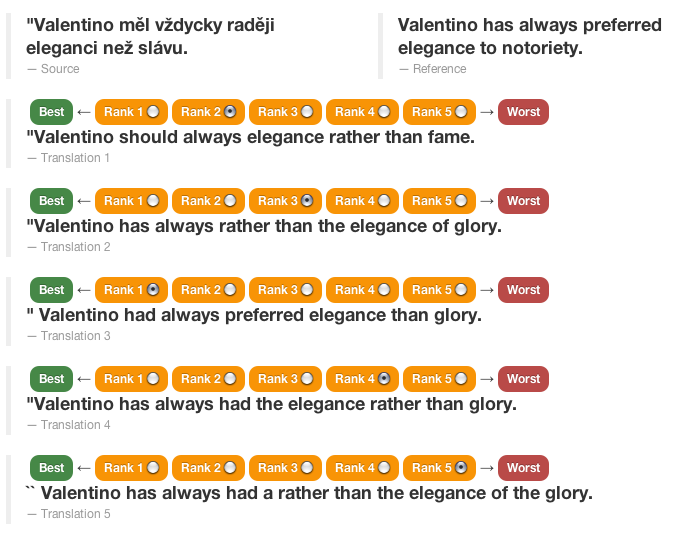
\includegraphics[width=6cm]{rankingtask.png}
    \end{center}
\end{frame}

    
\begin{frame}{SegRanks - Proposed Method}
    \begin{itemize}
        \item Split sentences into shorter segments
        \item Merge identical candidate segments produced by different systems
        \item Rank translations (relatively to each other) of each source segment separately
    \end{itemize}
    \begin{center}
        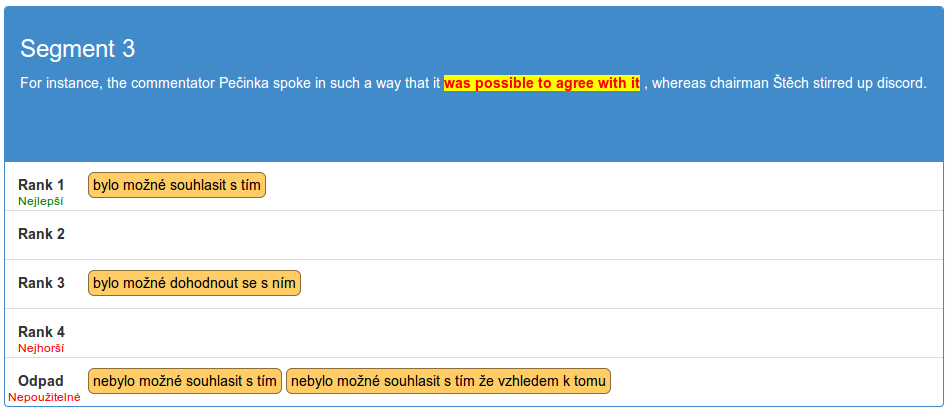
\includegraphics[width=10cm]{screenshot-small.png}
    \end{center}
\end{frame}

\begin{frame}{Segment Extraction}
    \begin{center}
        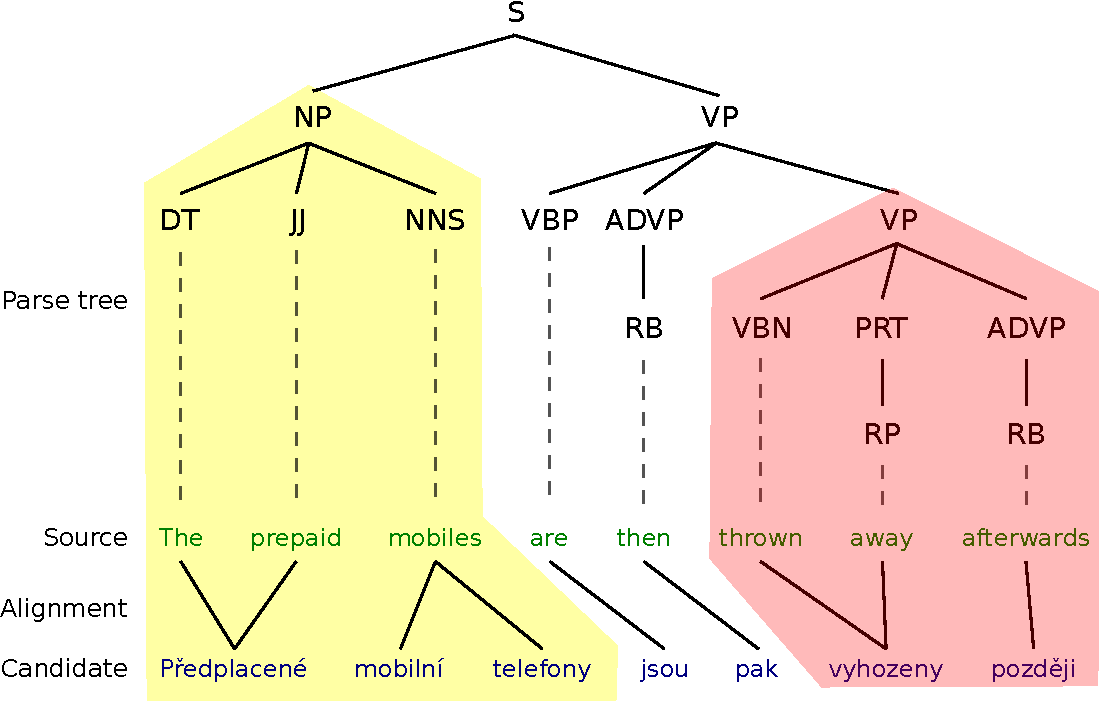
\includegraphics[width=10cm]{tree-align.pdf}
    \end{center}
\end{frame}

%\begin{frame}{Segranks annotation interface}
    %\begin{center}
        %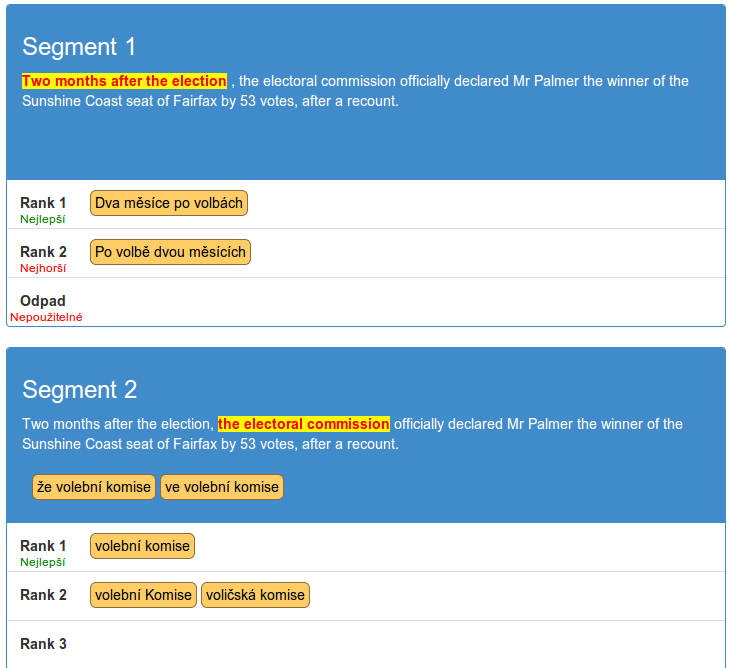
\includegraphics[width=8cm]{segranks-screenshot.png}
    %\end{center}
%\end{frame}

\begin{frame}{Experiments 1/4}
    \begin{itemize}
        \item A large evaluation experiment on EN-CS WMT14 data conducted
        \item The overall ranking of MT systems obtained by this method is very similar
            to the official WMT system ranking
        \item To estimate robustness of the annotation method, I measured annotator agreements
    \end{itemize}
    \begin{cvarblock}[8cm]{Annotator Agreements}
    \begin{center}
        \begin{tabular}{r|cc}
            & WMT official & SegRanks \\
            \hline
            intra-annotator $\kappa$ & 0.448 &  0.593      \\
            inter-annotator $\kappa$ & 0.360 &  0.397      \\
        \end{tabular}
    \end{center}
    \end{cvarblock}
\end{frame}

\begin{frame}{Experiments 2/4}
    \begin{itemize}
        \item Reuse the collected annotations to evaluate new, unseen sentences
        \item 58.8 \% of segments of unseen sentences were already annotated
        \vspace{0.5em}
        \item Computing system scores using only matched segments does not work
        \begin{itemize}
            \item Systems are more likely to agree on better translations 
            \item Unseen systems are very overestimated
        \end{itemize}
    \end{itemize}
\end{frame}

\begin{frame}{Experiments 3/4}
    \begin{itemize}
        \item The task is to extrapolate ranks of the unseen segments
        \item Take the rank of the closest segment (KNN for $k=1$)
        \item Does not work, the closest segments are usually better
    \end{itemize}
    \begin{center}
        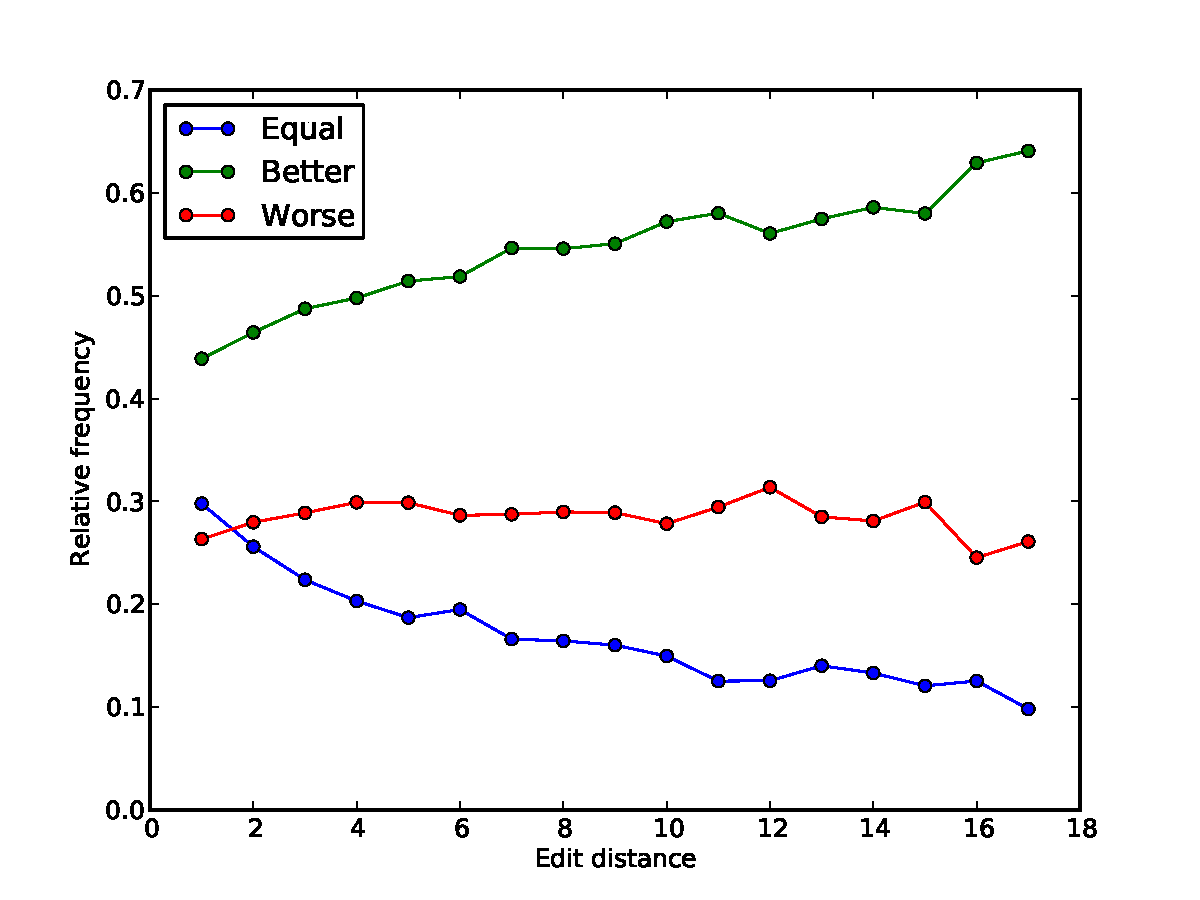
\includegraphics[width=8cm]{per-distance.pdf}
    \end{center}
\end{frame}

\begin{frame}{Experiments 4/4}
    \begin{itemize}
        \item Use the collected annotations to tune a statistical MT system
        \item \textbf{Minimum Error Rate Training} finds optimal weights of loglinear model
    \end{itemize}
    \begin{cvarblock}{Results}
        \begin{center}
  \begin{tabular}{r|c|cc|cc}
    & \textbf{\#Mert} & \multicolumn{2}{|c|}{\textbf{Automatic}} & \multicolumn{2}{|c}{\textbf{Manual}} \\
    & \textbf{iter-} & \multicolumn{2}{|c|}{\textbf{Evaluation}} & \multicolumn{2}{|c}{\textbf{Evaluation}} \\
    \textbf{Tunable metric} & \textbf{ations} & \textbf{BLEU} & \textbf{CDER}  & \textbf{Better} & \textbf{Worse} \\
    \hline
    \metric{BLEU} (baseline) & 11 & \textbf{0.1782} & \textbf{0.3855} & --- & --- \\
    \metric{ExactMatch}      & 20 & 0.1637 & 0.3674 & 22 \% & 38 \% \\
    \metric{PenalizeUnknown} &  8 & 0.1772 & 0.3850 & \textbf{34 \%} & \textbf{25 \%} \\
    \metric{SegRanksBLEU}    &  8 & 0.1753 & 0.3835 & 29 \% & 49 \% \\
  \end{tabular}
        \end{center}
    \end{cvarblock}
\end{frame}
    
\begin{frame}{Metrics Task in a Nutshell}
    \vspace{-0.5em}
    \begin{center}
%    \includegraphics<2>[width=10cm]{metrics-task-diagram-1.png}
%    \includegraphics<3>[width=10cm]{metrics-task-diagram-2.png}
%    \includegraphics<4>[width=10cm]{metrics-task-diagram-3.png}
%    \includegraphics<5>[width=10cm]{metrics-task-diagram-4.png}
%    \includegraphics<6>[width=10cm]{metrics-task-diagram-5.png}
%    \includegraphics<7>[width=10cm]{metrics-task-diagram-6.png}
    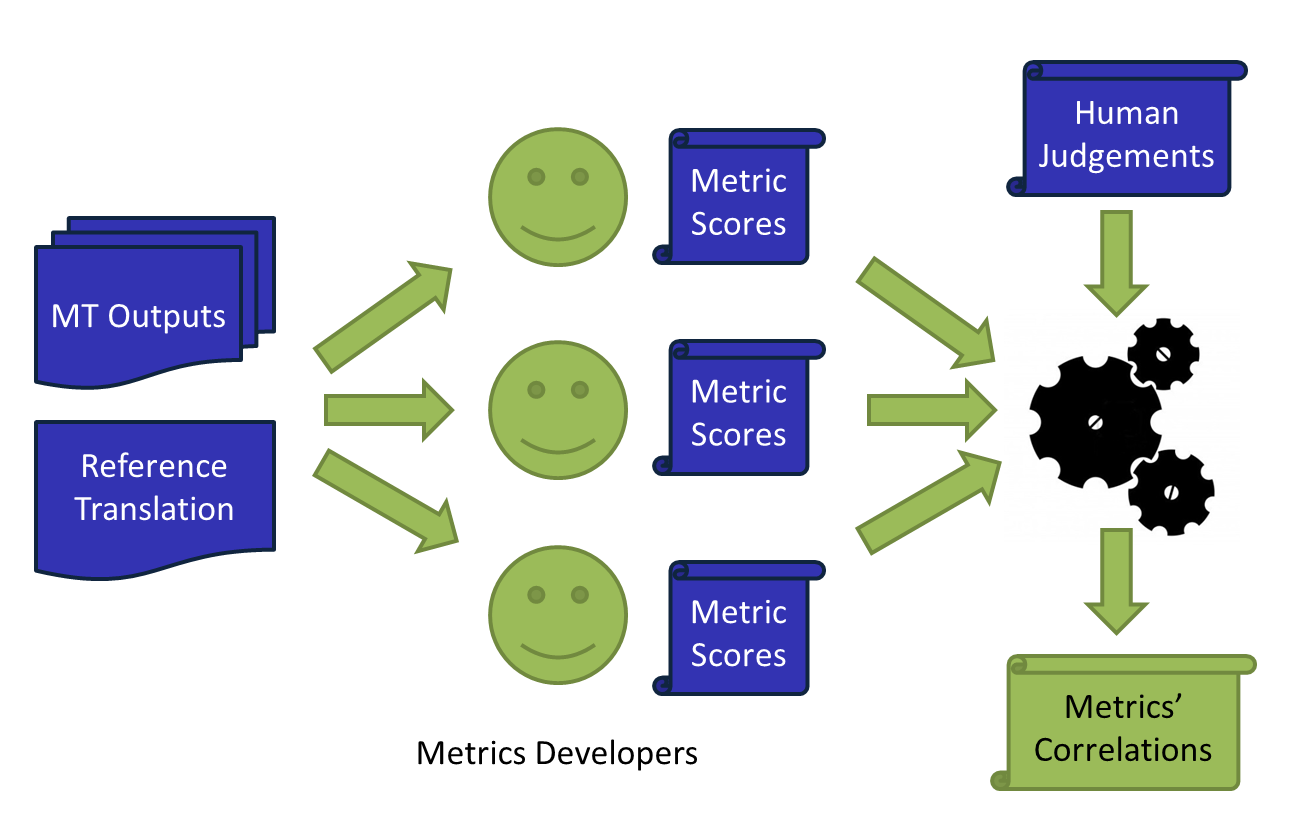
\includegraphics[width=10cm]{metrics-task-diagram-6.png}
   \end{center}
\end{frame}

\begin{frame}{Two subtasks}
    %\pause
    \begin{columns}[T]
        \begin{column}{8cm}
          \begin{itemize}
              \item \textbf{System level}
            \begin{itemize}

              \item Participants compute one score for the whole test set, as
                  translated by each of the systems
              \item Pearson correlation coefficient between these scores and
                  official human scores is computed
            \end{itemize}
          \end{itemize}
      \end{column}
      \begin{column}{3cm}
          \begin{center}
            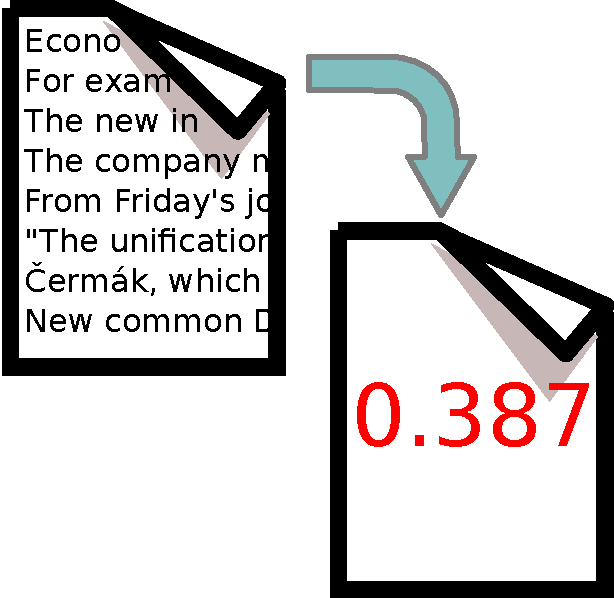
\includegraphics[width=2.5cm]{segment.pdf}
          \end{center}
      \end{column}
  \end{columns}
  %\pause
  \vspace{0.5em}
  \begin{columns}
      \begin{column}{8cm}
          \begin{itemize}
              \item \textbf{Sentence level}
            \begin{itemize}
              \item Participants compute one score for each sentence of
                  each system's translation
              \item Kendall's $\tau$ correlation coefficient of pairwise comparisons given
                  by humans and the metric is computed
            \end{itemize}
          \end{itemize}
      \end{column}
      \begin{column}{3cm}
          \begin{center}
            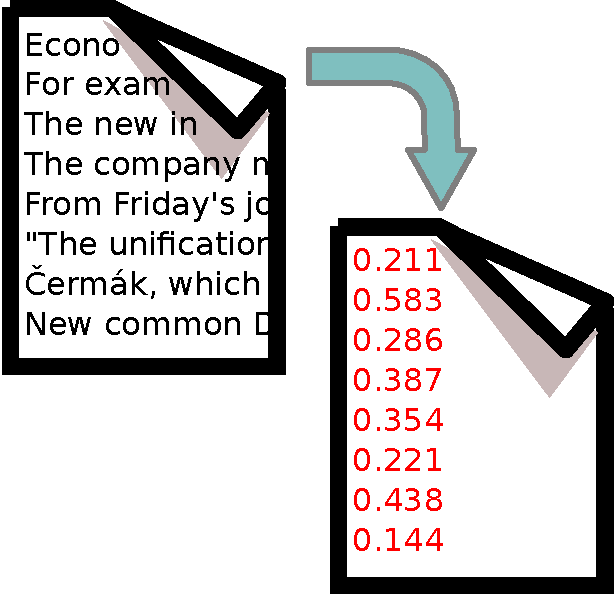
\includegraphics[width=2.5cm]{system.pdf}
          \end{center}
      \end{column}
  \end{columns}
\end{frame}

\begin{frame}{Metrics Task Summary}
    \begin{itemize}
        \item 23 metrics from 12 research groups, 6 baseline metrics
        \begin{itemize}
            \item Most of them are described in the thesis
        \end{itemize}
        \vspace{0.5em}
        \item Introduced and discussed several changes towards fairer metaevaluation
        \begin{itemize}
            \item Changed correlation measure in the system level task
            \item Metric ties considered neither concordant nor discordant in the sentence level
        \end{itemize}
        \vspace{0.5em}

        \item Scripts published together with human judgments
        \begin{itemize}
            \item Anyone can reproduce the results and use it to evaluate new metrics
        \end{itemize}
        \vspace{0.5em}
        \item Chef's tips for metric developers:
        \begin{itemize}
            \item Use features from various linguistic layers
            \item Tune parameters of your metric
        \end{itemize}
          \hfill\raisebox{0pt}[0pt][0pt]{
\includegraphics[width=2cm]{chef_says_okay.png}}
    \end{itemize}
\end{frame}


%\def\hi#1{\textbf{\textcolor{blue}{#1}}}
%\begin{frame}{System-Level Correlations into English}
%  \vspace{-0.5em}
%  \begin{center}
%  \footnotesize
%    \begin{tabular}{r|cccccc}
%\textbf{From} & \textbf{fr} & \textbf{de} & \textbf{hi} & \textbf{cs} & \textbf{ru} & \textbf{Avg} \\
%\hline
%
% \metric{DiscoTK-party-tuned} & \rangeA{.98}        & \best{\rangeB{.94}} & \rangeA{.96}        & \rangeA{.97}        & \best{\rangeC{.87}} & \best{\rangeB{.94}}\\
% \metric{LAYERED}             & \rangeA{.97}        & \rangeC{.89}        & \best{\rangeA{.98}} & \rangeB{.94}        & \rangeC{.85}        & \rangeB{.93}      \\
% \metric{DiscoTK-party}       & \rangeA{.97}        & \rangeB{.92}        & \rangeC{.86}        & \rangeA{.98}        & \rangeC{.86}        & \rangeB{.92}       \\
% \metric{UPC-STOUT}           & \rangeA{.97}        & \rangeB{.91}        & \rangeC{.90}        & \rangeB{.95}        & \rangeD{.84}        & \rangeB{.91}       \\
% \metric{VERTa-W}             & \rangeA{.96}        & \rangeC{.87}        & \rangeB{.92}        & \rangeB{.93}        & \rangeD{.85}        & \rangeB{.91}       \\
% \metric{VERTa-EQ}            & \rangeA{.96}        & \rangeC{.85}        & \rangeB{.93}        & \rangeB{.94}        & \rangeD{.84}        & \rangeB{.90}       \\
% \metric{tBLEU}               & \rangeA{.95}        & \rangeD{.83}        & \rangeA{.95}        & \rangeA{.96}        & \rangeD{.80}        & \rangeC{.90}       \\
% \metric{BLEU-NRC}            & \rangeA{.95}        & \rangeD{.82}        & \rangeA{.96}        & \rangeB{.95}        & \rangeE{.79}        & \rangeC{.89}       \\
% \baseline{BLEU}                & \rangeA{.95}        & \rangeD{.83}        & \rangeA{.96}        & \rangeB{.91}        & \rangeE{.79}        & \rangeC{.89}       \\
% \metric{UPC-IPA}             & \rangeA{.97}        & \rangeC{.89}        & \rangeB{.91}        & \rangeD{.82}        & \rangeD{.81}        & \rangeC{.88}       \\
% \baseline{CDER}                & \rangeA{.95}        & \rangeD{.82}        & \rangeD{.83}        & \rangeA{.97}        & \rangeD{.80}        & \rangeC{.87}       \\
% \metric{APAC}                & \rangeA{.96}        & \rangeD{.82}        & \rangeE{.79}        & \rangeA{.98}        & \rangeD{.82}        & \rangeC{.87}       \\
% \metric{REDSys}              & \best{\rangeA{.98}} & \rangeC{.90}        & \rangeF{.68}        & \rangeA{.99}        & \rangeD{.81}        & \rangeC{.87}       \\
% \metric{REDSysSent}          & \rangeA{.98}        & \rangeB{.91}        & \rangeF{.64}        & \best{\rangeA{.99}} & \rangeD{.81}        & \rangeC{.87}       \\
% \baseline{NIST}                & \rangeA{.96}        & \rangeD{.81}        & \rangeE{.78}        & \rangeA{.98}        & \rangeD{.80}        & \rangeC{.87}       \\
% \metric{DiscoTK-light}       & \rangeA{.96}        & \rangeB{.93}        & \rangeF{.56}        & \rangeA{.95}        & \rangeE{.79}        & \rangeD{.84}       \\
% \metric{Meteor}              & \rangeA{.98}        & \rangeB{.93}        & \rangeF{.46}        & \rangeA{.98}        & \rangeD{.81}        & \rangeD{.83}       \\
% %\metric{TER}                 & \rangeA{.95}        & \rangeE{.77}        & \rangeF{.62}        & \rangeA{.98}        & \rangeD{.81}        & \rangeD{.83}      \\
% \baseline{WER}                 & \rangeA{.95}        & \rangeE{.76}        & \rangeF{.61}        & \rangeA{.97}        & \rangeD{.81}        & \rangeD{.82}       \\
% \metric{AMBER}               & \rangeB{.95}        & \rangeB{.91}        & \rangeF{.51}        & \rangeF{.74}        & \rangeE{.80}        & \rangeE{.78}       \\
% %\metric{PER}                 & \rangeB{.95}        & \rangeC{.87}        & \rangeF{.41}        & \rangeC{.88}        & \rangeE{.80}        & \rangeE{.78}      \\
% \metric{ELEXR}               & \rangeA{.97}        & \rangeC{.86}        & \rangeF{.54}        & \rangeB{.94}        & \rangeF{-.40}       & \rangeF{.58}       \\
%% XXX Metriky TER a PER jsou schovany, nevadi?
%
%    \end{tabular}
%  \end{center}
%\end{frame}

\end{document}
